\subsection{Komplexität mit TBoxen, obere
Schranke}\label{komplexituxe4t-mit-tboxen-obere-schranke}

\subsubsection{Obere Schranke}

Wir wollen zeigen:

\begin{theorem}
In $\ALC$ ist die Erfüllbarkeit von Konzepten bzgl. TBoxen
ExpTime-Vollständig.
\end{theorem}

Mit Lemma 2.9: Subsumtion und Äquivalenz ExpTime-Vollständig.

Wir beginnen mit oberer Schranke (Enthaltensein in ExpTime):

\begin{itemize}
  \item wir verwenden ein Verfahren aus der Modallogik: Typelimination
  \item basiert auf syntaktischem Typ-Begriff
\end{itemize}

\subsubsection{Syntaktische Typen}\label{synt-typ}

Wir nehmen an, dass das Eingabe-Konzept $C_0$ in NNF ist und die Eingabe-TBox die Form $\{\top \sqsubseteq C_{\MT}\}$ hat mit $C_{\MT}$ in NNF.

\begin{definition}{Typ}

Ein Typ für $C_{0}$ und $T$ ist Teilmenge
$t \subseteq sub\left( C_{0},T \right)$, so dass

\begin{enumerate}
\def\labelenumi{\arabic{enumi}.}
\item
  $A \in t$ gdw. $\neg A \notin t$ für alle
  $\neg A \notin sub\left( C_{0},T \right)$
\item
  $C \sqcap D \in t$ gdw. $C \in t$ und $D \in t$ für alle
  $C \sqcap D \in sub\left( C_{0},T \right)$
\item
  $C \sqcup D \in t$ gdw. $C \in t$ oder $D \in t$ für alle
  $C \sqcup D \in sub\left( C_{0},T \right)$
\item
  $C_{T} \in t$
\end{enumerate}
\end{definition}

\textbf{T5.1}

Beispiel:

$C_0 = A$, $\MT = \{\top \subseteq C_{\MT}\}$ mit $$C_{\MT} = \exists r.\exists r.A \sqcap \forall r.A' \sqcap (\neg A \sqcup \neg A')$$

Dann ist $$sub(C_0, \MT) = \{A, C_{\MT}, \exists r.\exists r.A, \forall r.A',\neg A \sqcup \neg A', \exists r.A, A', \neg A, \neg A'\}$$

Sei $M = \{C_{\MT}, \exists r.\exists r. A, \forall r.A', \neg A \sqcup \neg A'\}$

Die Typen für $C_0$ und $\MT$ sind:

\begin{itemize}
  \item $t_0 = M \cup \{\neg A, \neg A'\}$
  \item $t_1 = M \cup \{\neg A, A'\}$
  \item $t_2 = M \cup \{A, \neg A'\}$
  \item $t_0' = M \cup \{\exists r.A\}$
  \item $t_1' = M \cup \{\exists r.A\}$
  \item $t_2' = M \cup \{\exists r.A\}$
\end{itemize}

\subsubsection{Typelimination}\label{typelimination}

Die generelle Idee der Typelimination bei Eingabe $C_0$, $\MT$:

\begin{enumerate}
\def\labelenumi{\arabic{enumi}.}
\item
  Generiere alle Typen für $C_{0}$ und $T$ (exponentiell viele)
\item
  Eliminiere wiederholt Typen, die in keinem Modell von $T$ vorkommen
  können
\item
  Überprüfe, ob ein Typ überlebt hat, der $C_{0}$ enthält
\item
  Wenn ja, antworte „erfüllbar``, sonst „unerfüllbar``
\end{enumerate}

\subsubsection{Schlechte Typen}\label{schlechter-typ}

Wir formalisieren ``Typen, die in keinem Modell vorkommen können''.

\begin{definition}{schlechter Typ}

Sei $\Gamma$ Typenmenge und $t \in \Gamma$.

Dann ist $t$ \emph{schlecht in} $\Gamma$, wenn für ein $\exists r.C \in t$ gilt:

\begin{center}Es gibt kein $t^{'} \in \Gamma$ mit
$\left\{ C \right\} \cup \left\{ \text{D\ } \middle| \ \forall r.D \in t \right\} \subseteq t^{'}$.\end{center}
\end{definition}

Erklärung: $t$ braucht einen ``Zeugen'', es gibt aber keinen
geeigneten.

\textbf{T5.1cont}

Beispielsweise ist $t_0'$ schlecht in der Menge $\{t_0,t_1,t_2,t_0',t_1',t_2'\}$. Für $\exists r.A \in t_0'$ ist die Menge aus Definition 5.3 $\{A,A'\}$. Kein Typ enhält $A$ und $A'$. Analog: $t_1'$, $t_2'$ sind schlecht. Entfernt man diese drei so erhält man die Menge $\Gamma_1 = \{t_1,t_2,t_2\}$. 

Nun sind aber $\{t_1,t_2,t_3\}$ schlecht in $\Gamma_1$: Sie enthalten $\exists r. \exists r.A$ , aber kein Typ in $\Gamma_1$ enthält $\exists r.A$.

\begin{proposition}
$\ALC$-Elim($C_0,\MT$) terminiert nach $2^{\mathcal{O}(|C_0|+|\MT|)}$ Schritten.
\end{proposition}

\textbf{T5.2}

\begin{proof}
Sei $n = \left| C_{0} \right| + |T|$. Proposition folgt aus:

\begin{enumerate}
\def\labelenumi{\arabic{enumi}.}
\item
  Es gibt nur $2^{n}$ Typen mit $n \left| C_{0} \right| + T$
  (\protect\hyperlink{lemma-3.15}{Lemma 3.15})
\item
  In jedem Schritt, der repeat-Schleife wird mindestens ein Typ
  eliminiert; die Schleife terminiert spätestens nach $2^{n}$
  Durchläufen.
\item
  Die restlichen Operationen (prüfen, ob ein Typ schlecht ist usw.)
  können leicht in Zeit $2^{O\left( n \right)}$ implementiert werden.
\end{enumerate}
\end{proof}

\begin{proposition}
$\ALC$-Elim($C_0,\MT$) antwortet ``erfüllbar'' gdw. $C_0$ erfüllbar bzgl. $\MT$
\end{proposition}

\textbf{T5.3}. 

\textbf{Korrekt}

Per Induktion über Struktur von $C$.

Antworte $\text {$\ALC$}\mathrm{-}Elim(C_{0},T)$ „erfüllbar`` und sei
$\Gamma_{i}$ die resultierende Typmenge. Dann gibt es
$t_{0} \in \Gamma_{i}$ mit $C_{0} \in t_{0}$. Definiere
Interpretation $\MI$:

\begin{itemize}
\item
  $\Delta^{\MI} = \Gamma_{i}$
\item
  $A^{\MI} = \left\{ t \in \Gamma_{i} \middle| A \in t \right\}$
\item
  $r^{i} = \left\{ \left( t,t^{'} \right)\in \Gamma_i \times \Gamma_i\  \middle| \ \forall r.C \in t\ \mathrm{\text{impliziert}}\ C \in t^{'} \right\}$
\end{itemize} 

\paragraph{Beispiel}

$C_0 = A$, $\MT = \{\top \sqsubseteq \forall r.\exists r.A \sqcap (\neg A \sqcup \exists r.A\}$

$sub(C_0, \MT) = \{A,C_{\MT}, \forall r.\exists r.A, \neg A \sqcup \exists r.A, \exists r.A, \neg A\}$

Sei $M = \{C_{\MT}, \forall r.\exists r.A, \neg A \sqcup \exists r.A\}$ 

Typen:

\begin{itemize}
  \item $t_0 = M \cup \{\neg A\}$
  \item $t_1 = M \cup \{A,\exists r.A\}$
  \item $t_1 = M \cup \{\neg A,\exists r.A\}$
\end{itemize}

Keine der Typen ist schlecht. Also $\Gamma_1 = \{t_0,t_1,t_2\}$

Interpretation $\MI$:

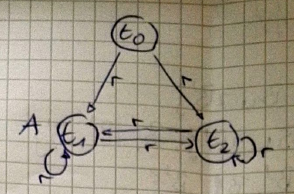
\includegraphics[width=3.71910in,height=2.33200in]{media/52typelim.png}

\paragraph{Beweis}

Zu zeigen: $\MI$ ist Modell von $C_{0}$ und $\MT$ *.

Behauptung: Für alle $C \in sub\left( C_{0},\MT \right)$ und alle
$t \in \Gamma_{i}$:
$$C \in t \Rightarrow t \in C^{\MI}$$

Daraus folgt:

\begin{enumerate}
\def\labelenumi{\arabic{enumi}.}
\item
  * Wegen $C_{0} \in t_{0}$ ist $t_{0} \in C_{0}^{\MI}$
\item
  Wegen $C_{T} \in t$ für alle $t \in \Gamma_{i}$ folgt
  $t \in C_{T}^{\MI}$. für alle $t \in \Gamma_{i}$ Also ist $\MI$ Modell von $\MT$.
\end{enumerate}

\textbf{I.A.} $C = A$. Folgt direkt aus Definition $\MI$.

$C = \neg A$. Nach Definition „Typ`` gilt $A \notin t$. Nach
Definition $\MI$ ist $t \notin A^{\MI}$.

\textbf{I.S.} Fallunterscheidung:

\begin{itemize}
\item
  $C = D \sqcap D^{'}$

Nach Definition „Typ`` ist $D \in t$ und $D^{'} \in t$. Nach
\textbf{I.V}.: $t \in D^{\MI}$ und $t \in \left( D^{'} \right)^{\MI}$.
Nach Semantik: $t \in \left( D \sqcap D^{'} \right)^{\MI}$.

\item
  $C = D \sqcup D^{'}$

Analog.

\item
  $C = \forall r.D$

Sei $\forall r.D \in t$ und $\left( t,t^{'} \right) \in r^{\MI}$. Nach
Definition $r^{\MI}$ muss $D \in t^{'}$ gelten. Nach \textbf{I.V}.:
$t^{'} \in D^{\MI}$, also $t \in \left( \forall r.D \right)^{\MI}$

\item
  $C = \exists r.D$

Sei $\exists r.D \in t$. Da $t \in \Gamma_{i}$ (also nicht
schlecht), gibt es $t^{'} \in \Gamma_{i}$ mit $D \in t^{'}$ und
$E \in t^{'}$ für alle $\forall r.E \in t$. Nach \textbf{I.V.} gilt
$t^{'} \in D^{\MI}$ und nach Definition von $r^{\MI}$ gilt
$\left( t,t^{'} \right) \in r^{\MI}$. Also
$t \in \left( \exists r.D \right)^{\MI}$
\end{itemize}

\textbf{Vollständigkeit}. 

Beweisskizze per Induktion über i.

Sei $C_{0}$ erfüllbar bzgl. $\MT$ und sei $\MI$ Modell von $\MT$ mit
$d_{0} \in C_{0}^{\MI}$. 

Sei $\Gamma = \left\{ t_{\MI}\left( d \right)\  \middle| \ d \in \Delta^{\MI} \right\}$.

Sei $\Gamma_{0},\ldots,\Gamma_{k}$ die von $\text {$\ALC$}\mathrm{-}\text{Elim}\left( C_{0},\MT \right)$ erzeugte Sequenz. 

Behauptung: $\Gamma \subseteq \Gamma_{i}$ für alle $i \geq 0$

Daraus folgt wegen $d_{0} \in C_{0}^{\MI}$, dass $C_{0} \in t_{i}\left( d_{0} \right) \in \Gamma \subseteq \Gamma_{k}$.

Also gibt $\text {$\ALC$}\mathrm{-}Elim(C_{0},\MT)$ „erfüllbar`` zurück.

I.A. $i = 0$. Einfach jedes Element von $\Gamma$ (semantisch Typ)
ist auch ein syntaktischer Typ.

I.S. Gelte $\Gamma \subseteq \Gamma_{i}$ (I.V.). Zu zeigen:
$\Gamma \subseteq \Gamma_{i + 1}$. 

Sei $t \in \Gamma$. Es genügt zu zeigen: $t$ ist nicht schlecht in $\Gamma_{i}$. 

Sei $\exists r.C \in t$ und $S = \left\{ C \right\} \cup \left\{ D \middle| \forall r.D \in T \right\}$.

Da $t \in \Gamma$, gibt es $d \in \Delta^{\MI}$ mit $t_{\MI}\left( d \right) = t_{0}$. 

Also gibt es nach Semantik $e \in \Delta^{\MI}$, $\left( d,e \right) \in r^{\MI}$, $e \in D^{\MI}$ für alle $D \in S$

$t's$ gilt also $S \subseteq t_{\MI}\left( e \right)$ und $t_{\MI}\left( e \right) \in \Gamma \subseteq \Gamma_{i}$. Es folgt:
$t$ nicht schlecht

\begin{theorem}
In $\ALC$ ist die Erfüllbarkeit von Konzepten bzgl. TBoxen entscheidbar in ExpTime.
\end{theorem}

\subsubsection{Zusammenhang mit Tableau-Algorithmen}

Offensichtliche Entsprechungen:

\begin{itemize}
  \item $\sqcap$-Regel, $\sqcup$-Regel, TBox-Regel finden sich wieder in der Definition eines Typs.
  \item $\exists$-Regel und $\forall$-Regel finden sich wieder in Def. von ``schlecht''.
  \item Freiheit von offensichtlichen Widersprüchen findet sich wieder in der Definition eines Typs
\end{itemize}

Unterschiede:

\begin{itemize}
  \item Tableau-Algorithmus benötigt im Worst Case dreifach exponentielle Laufzeit
  \item Typelimination benötigt im Best Case exponentielle Laufzeit
\end{itemize}

\subsection{Komplexität mit TBoxen, untere Schranke}\label{komplexituxe4t-mit-tboxen-untere-schranke}

Um die ExpTime-Härte zu zeigen, reduzieren wir auf ein spieltheoretisches Problem:

\subsubsection{ExpTime-Spiele}\label{exptime-spiele}

\begin{itemize}
\item
  Zwei Spieler spielen auf gegebener aussagenlogischen Formel
  $\varphi$
\item
  Jede Variable in $\varphi$ gehört entweder Spieler 1 oder Spieler 2
\item
  Das Spiel beginnt auf einer gegebenen Anfangsbelegung $\pi_{0}$ der
  Variablen
\item
  Spieler 1 beginnt, die Spieler wechseln sich ab
\item
  In jedem Zug ändert Spieler Wahrheitswert einer seiner Variablen; es
  ist erlaubt, zu passen
\item
  Spieler 1 gewinnt, wenn $\varphi$ jemals wahr wird (egal, welcher
  Spieler gezogen hat)
\item
  Spieler 2 gewinnt, wenn das Spiel unendlich weitergeht ohne dass
  $\varphi$ wahr wird
\end{itemize}

\begin{definition}{ExpTime-Spiele}

\begin{itemize}
\item
  \emph{Spiel}: Tupel
  $\left( \varphi,\ \Gamma_{1},\Gamma_{2},\pi_{0} \right)$ mit
  $\Gamma_{1},\Gamma_{2}$ Partitionierung der Variablen in
  $\varphi_{1}$ und $\pi_{0}$ Anfangsbelegung
\item
  \emph{Konfiguration}: Paar $(i,\pi)$ mit
  $i \in \left\{ 1,2 \right\}$ aktiver Spieler und $\pi$ Belegung
\item
  $\pi$ ist $j$-\emph{Variation} von $\pi'$
  $\left( j \in \left\{ 1,2 \right\} \right)$ wenn $\pi = \pi'$ oder
  $\pi$ und $\pi^{'}$ unterscheiden sich nur in einer Variablen
  $p \in \Gamma_{j}$
\end{itemize}
\end{definition}

„$\pi$ ist $j$-Variation von $\pi'$`` bedeutet: Spieler $j$ kann
$\pi$ in $\pi'$ transformieren (oder umgekehrt).

Das hier relevante Entscheidungsproblem bezieht sich auf \emph{Gewinnstrategien} für Spieler 2.

\subsubsection{Gewinnstrategie}\label{definition-5.8-gewinnstrategie}

Intuitiv:

\begin{itemize}
  \item eine Gewinnstrategie sagt Spieler 2 nach jedem möglichen Spielverlauf wie er spielen muss um zu gewinnen.
  \item wenn Spieler 2 eine Gewinnstrategie hat, so kann er das Spiel gewinnen
\end{itemize}

\begin{definition}{Gewinnstrategie}

Gewinnstrategie für Spieler 2 in Spiel
$\left( \varphi,\Gamma_{1},\Gamma_{2},\pi_{0} \right)$ ist unendlicher
knotenbeschrifteter Baum $(V,E,l)$, wobei $l$ jedem Knoten
$v \in V$ Konfiguration $l(v)$ zuweist so, dass

\begin{enumerate}
\def\labelenumi{\alph{enumi})}
\item
  Wurzel beschriftet mit $\left( 1,\pi_{0} \right)$
\item
  wenn $l\left( v \right) = (2,\pi)$, dann hat $v$ Nachfolger
  $v^{'}$ mit $l\left( v' \right) = \left( 1,\pi^{'} \right)$, wobei
  $\pi^{'}$ $2$-Variation von $\pi$
\item
  wenn $l\left( v \right) = (1,\pi)$, dann hat $v$ Nachfolger
  $v_{0},\ldots,v_{\left| \Gamma_{1} \right|}$ mit
  $l\left( v_{1} \right) = (2,\pi_{i})$ wobei
  $\pi_{0},\ldots,\pi_{\left| \Gamma_{1} \right|}$ alle existierenden
  $1$-Variationen von $\pi$
\item
  wenn $l\left( v \right) = (i,\pi)$, dann nicht
  $\pi \vDash \varphi$
\end{enumerate}
\end{definition}

\subsubsection{ExpTime-Spiele als Entscheidungsproblem}

\begin{definition}

\emph{Spiel\textsubscript{1}} ist das folgende Problem: Gegeben Spiel
$\left( \varphi,\Gamma_{1},\Gamma_{2},\pi_{1} \right)$, entscheide ob
Spieler 2 eine Gewinnstrategie hat.
\end{definition}

\begin{theorem}
Spiel\textsubscript{1} ist ExpTime-Vollständig
\end{theorem}

Wir wollen nun die ExpTime-Härte von Erfüllbarkeit in $\ALC$ bzgl. TBoxen auf Spiel\textsubscript{1} reduzieren

\subsubsection{Reduktion}\label{reduktion}

Reduziere Spiel\textsubscript{1}: Gegeben Spiel
$\left( \varphi,\Gamma_{1},\Gamma_{2},\pi_{0} \right)$, konstruiere in
Polynomialzeit Konzept $C_{S}$ und TBox $\MT_{S}$ so, dass: 

\begin{lemma}Spieler 2 hat Gewinnstrategie in $S$ gdw. $C_{S}$ erfüllbar bzgl. $\MT_{S}$.\end{lemma}

Idee: (Baum)-Modelle von $C_S$ und $\MT_S$ kodieren Gewinnstrategien.

Beweisskizze:

Details der Reduktion:

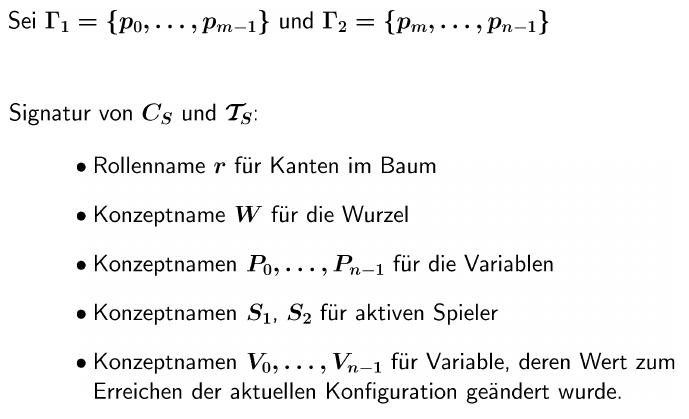
\includegraphics[width=3.71910in,height=2.33200in]{media/5red1.png}

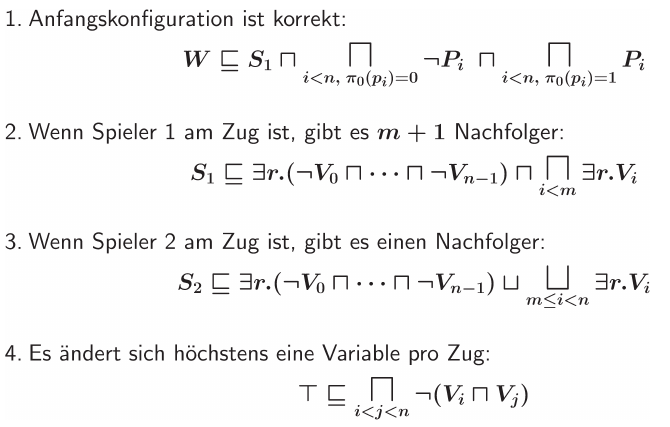
\includegraphics[width=3.71910in,height=2.33200in]{media/5red2.png}

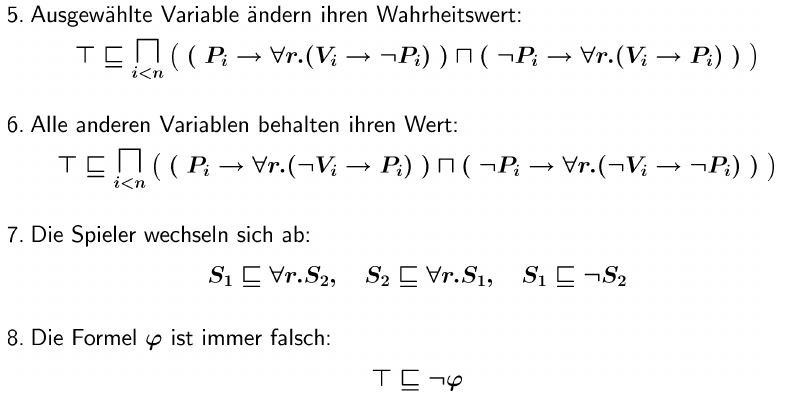
\includegraphics[width=3.71910in,height=2.33200in]{media/5red3.png}

Setze $C_S = W$ 

\begin{itemize}
\item
  Hinrichtung: Erzeuge aus der Gewinnstrategie Interpretation und zeige, dass diese Modell ist.
\item
  Rückrichtung: Nimm an es gibt Baummodell und erzeuge daraus
  Gewinnstrategie.
\end{itemize}

\begin{theorem}
In $\ALC$ ist die Erfüllbarkeit von TBoxen ExpTime-hart.
\end{theorem}

Daraus ergibt sich zusammen mit \protect\hyperlink{theorem-5.6}{Theorem 5.6} ExpTime-Vollständigkeit.

\subsection{Komplexität ohne TBoxen obere
Schranke}\label{komplexituxe4t-ohne-tboxen-obere-schranke}

\subsubsection{Obere Schranke}

Wir wollen zeigen:

\begin{theorem}
In $\ALC$ ist die Erfüllbarkeit von Konzepten (ohne TBoxen)
PSpace-Vollständig.
\end{theorem}

Mit Lemma 2.8 sind dann auch Subsumtion und Äquivalenz PSpace-vollständig.

\subsubsection{ALC-Worlds}\label{alc-worlds}

Wenn $C$ erfüllbar, dann hat $C$ ein Baummodell (Theorem 3.4). Ohne TBox ist dessen Tiefe mit $\left| C \right|$ beschränkt. 

In PSpace:

\begin{itemize}
\item
  Ein linear Tiefer Baum ist exponentiell groß
\item
  Gesamtes Modell im Speicher: nicht PSpace
\item
  Stattdessen Prüfe Existenz des Baumes mittels Tiefensuche; halte zu
  jeder Zeit nur einen Pfad des Baumes im Speicher
\end{itemize}

\begin{theorem}
PSpace $=$ NPSpace
\end{theorem}

\begin{definition}{$i$-Konzepte}

Für $i \geq 0$ ist die Menge der $i$-Konzepte definiert als:
$$sub_{i} := \left( C_{0} \right) \left\{ C \in sub\left( C_{0} \right)\  \middle| \text{\ rd}\left( C \right) \leq i \right\}$$
\end{definition}

\begin{definition}{i-Typ}

Sei $i \geq 0$. $\MI$-Typ für $C_{0}$ ist Teilmenge
$t \subseteq sub_{i}\left( C_{0} \right)$ so, dass

\begin{enumerate}
\def\labelenumi{\arabic{enumi}.}
\item
  $A \in t$ gdw. $\neg A \notin t$ für alle
  $\neg A \in sub_{i}\left( C_{0} \right)$
\item
  $C \sqcap D \in t$ gdw. $C \in t$ und $D \in t$ für alle
  $C \sqcap D \in sub_{i}\left( C_{0} \right)$
\item
  $C \sqcup D \in t$ gdw. $C \in t$ oder $D \in t$ für alle
  $C \sqcup D \in sub_{i}\left( C_{0} \right)$
\end{enumerate}
\end{definition}

\paragraph{ALC-Worlds}\label{alc-worlds-1}

Rekursion über $\MI$-Typen.

\begin{proposition}
ALC-Worlds($C_{0}$) terminiert und benötigt polynomiellen Platz (in $|C_0|$).
\end{proposition}

Beweisskizze. Stelle als Rekursionsbaum dar. Verzweigungsgrad beschränkt
durch Anzahl der $\exists$. Tiefe Beschränkt durch $rd(C_{0})$. Der
Rekursionsstack hat höchstens Tiefe $\left| C_{0} \right|$ und der
Platzbedarf pro Aufruf ist polynomiell.

\subsubsection{Korrektheit und Vollständigkeit}\label{proposition-5.18}

\begin{proposition}
$\ALC$-Worlds($C_0$) = true gdw. $C_0$ erfüllbar
\end{proposition}


Korrektheitsbeweis per Induktion über $C_{0}$:

Zunächst definieren wir eine Interpretation $\MI$. Für jeden Knoten $v \in V_0 \setminus \{v_0\}$ sei $\sigma (v)$ der Rollenname $r$ des Konzeptes $\exists r.C$, für das der Aufruf $v$ gemacht wurde.

Definiere $\MI$ nun wie folgt:

\begin{itemize}
  \item $\Delta^{\MI} = V$
  \item $r^{\MI} = \{(v,v')\in E | \sigma (v') = r\}$
  \item $A^{\MI} = \{v | A \in p_1(v)\}$
\end{itemize}

($p_1(v)$ = 1. Parameter in $l(v)$)

Behauptung: Für alle $v \in V$ und $C \in sub(C_0)$ gilt $$C \in p_1(v)\ impliziert v \in C^{\MI}$$

Da $C_0 \in p_1(v_0)$ ist auch $v_0 \in C_0^{\MI}$; also ist $\MI$ ein Modell von $C_0$.

\textbf{T5.9a}

\textbf{I.A.} $C = A$. Folgt direkt aus Definition $\MI$.

$C = \neg A$. Da der Lauf erfolgreich ist, ist
$p_{1}\left( v \right)$ Typ für $C_{0}$. Nach Definition „Typ`` gilt
$A \notin p_{1}\left( v \right)$. Nach Definition $\MI$ ist
$v \notin A^{\MI}$.

\textbf{I.S.} Fallunterscheidung:

\begin{itemize}
\item
  $C = D \sqcap D^{'}$
\end{itemize}

Nach Definition „Typ`` ist $D \in p_{1}\left( v \right)$ und
$D^{'} \in p_{1}\left( v \right)$. Nach \textbf{I.V}.: $v \in D^{\MI}$
und $v \in \left( D^{'} \right)^{\MI}$. Nach Semantik:
$v \in \left( D \sqcap D^{'} \right)^{\MI}$.

\begin{itemize}
\item
  $C = D \sqcup D^{'}$
\end{itemize}

Analog.

\begin{itemize}
\item
  $C = \forall r.D$
\end{itemize}

Sei $\left( v,v^{'} \right) \in r^{\MI}$. Dann ist
$\left( v,v^{'} \right) \in E$ und $\sigma\left( v^{'} \right) = r$.
Wegen $\forall r.D \in p_{1}(v)$ ist auch
$D \in p_{1}\left( v^{'} \right)$. Nach I.V. gilt $v^{'} \in D$.
Also $v \in \left( \forall r.D \right)^{\MI}$

\begin{itemize}
\item
  $C = \exists r.D$
\end{itemize}

Ähnlich

\textbf{Beweis der Vollständigkeit}

Sei $C_0$ erfüllbar und $\MI$ ein Modell von $C_0$ und $d_0 \in C_0^{\MI.}$

Beweisidee:

Verwenden $\MI$, um die nichtdeterministischen Entscheidungen von $\ALC$-Worlds($C_0$) zu einem erfolgreichen Lauf zu ``lenken''.

\begin{theorem}
In $\ALC$ ist die Erfüllbarkeit von Konzepten in PSpace.
\end{theorem}

\subsection{Komplexität ohne TBoxen untere
Schranke}\label{komplexituxe4t-ohne-tboxen-untere-schranke}

\begin{definition}{PSpace-Spiel}

\begin{itemize}
\item
  \emph{Spiel}: Aussagenlogische Formel $\varphi$ mit Variablen
  $p_{1},\ldots,p_{n}$, $n$ gradzahlig
\item
  \emph{Konfiguration}: Wort $\pi \in \left\{ 0,1 \right\}*$
\end{itemize}
\end{definition}

\begin{definition}{Gewinnstrategie}

Gewinnstrategie für Spieler 1 in Spiel $\varphi$ ist endlicher
knotenbeschrifteter Baum $(V,E,L)$, wobei $l$ jedem Koten
$v \in V$ Konfiguration $l(v)$ zuweist, sodass
\end{definition}

\begin{enumerate}
\def\labelenumi{\alph{enumi})}
\item
  Wurzel beschriftet mit $\varepsilon$ (leere Konfiguration)
\item
  wenn $l\left( v \right) = w$ mit $\left| w \right|$ gerade und
  $\left| w \right| < n$ (Also Spieler 1 am Zug), dann hat $v$
  Nachfolger $v^{'}$ mit $l\left( v^{'} \right) \in \{ w0,w1\}$
\item
  wenn $l\left( v \right) = w$ mit \textbar{}w\textbar{} ungerade
  (also Spieler 2 am Zug), dann hat $v$ Nachfolger $v^{'}$ und
  $v''$mit $l\left( v^{'} \right) = w0$ und
  $l\left( v^{''} \right) = w1$
\item
  wenn $l\left( v \right) = w$ mit $\left| w \right| = n$, dann
  $w \vDash \varphi$
\end{enumerate}

\subsubsection{Theorem 5.25}\label{theorem-5.25}

In $\ALC$ ist die Erfüllbarkeit von Konzepten bzgl. leerer TBoxen
PSpace-Hart.

Beweisskizze. Konstruiere Konzept $C_{\varphi}$, so dass Spieler 1 hat
Gewinnstrategie in $\varphi$ gdw. $C_{\varphi}$ erfüllbar.

\subsection{Unentscheidbare
Erweiterungen}\label{unentscheidbare-erweiterungen}

\subsection{Konkrete Bereiche}\label{konkrete-bereiche}

Ein \emph{Konkreter Bereich} ist ein Paar $B = (\Delta^{B},\Phi^{B})$
wobei

\begin{itemize}
\item
  $\Delta^{B}$ eine Menge von \emph{Werten} ist und
\item
  $\Phi^{B}$ eine Menge von \emph{Prädikaten}
\end{itemize}

sodass jedes $P \in \Phi^{B}$ mit einer Stelligkeit $n \geq 0$
ausgestattet ist und mit einer Extension
$P^{B} \subseteq \left( \Delta^{B} \right)^{n}$.

\subsubsection{Definition 5.27 (ALCB
Syntax)}\label{definition-5.27-alcb-syntax}

Sei $B$ ein konkreter Bereich. Mit ALC($B$) bezeichnen wir die
Erweiterung von $\ALC$ um $B$, d.h. um

\begin{itemize}
\item
  \emph{Featurenamen} (eine zusätzliche Art von Rolle) und
\item
  die Konstruktoren $\exists R_{1},\ldots,\ R_{n}\text{.P}$ und
  $\forall R_{1},\ldots,R_{n}\text{.P}$
\end{itemize}

wobei $P \in \Phi^{B}$ $n$-Stellig ist und die $R_{i}$
\emph{Rollenkomposition} der Form $r_{1};\ldots;r_{k};f$ sind mit
$r_{j}$ Rollenname und $f$ Featurename.

\subsubsection{Definition 5.28 (ALCB
Semantik)}\label{definition-5.28-alcb-semantik}

Eine Interpretation $\MI$ ordnet nun zusätzlich zu jedem Featurenamen
$f$ eine Funktion $f^{\MI}:\Delta^{\MI} \rightarrow \Delta^{B}$ zu. Für
jede Rollenkomposition $r = r_{1};\ldots r_{k};f$ bezeichnet $R^{\MI}$
die Komposition der Interpretationen:
$R^{\MI} = r_{1}^{\MI} \circ \ldots \circ r_{k}^{\MI} \circ f$

Die Semantik der zusätzlichen Konstruktoren ist nun:

\[\left( \exists R_{1},\ldots,\ R_{k}\text{.P} \right)^{\MI} = \left\{ d \in \Delta^{\MI}\ |\ \exists d_{1},\ldots,d_{k}:\left( d,d_{i} \right) \in R_{i}^{\MI}\ \mathrm{fur}\ 1 \leq i \leq k\ \mathrm{\text{und}}\ \left( d_{1},\ldots,\ d_{k} \right) \in P^{B} \right\}\]

\[\left( \forall R_{1},\ldots,\ R_{k}\text{.P} \right)^{\MI} = \left\{ d \in \Delta^{\MI}\ |\ \forall d_{1},\ldots,d_{k}:\left( d,d_{i} \right) \in R_{i}^{\MI}\ \mathrm{fur}\ 1 \leq i \leq k\ \mathrm{\text{impliziert}}\ \left( d_{1},\ldots,\ d_{k} \right) \in P^{B} \right\}\]

\subsubsection{2-Registermaschinen}\label{registermaschinen}

\begin{itemize}
\item
  Endlich viele Zustände
\item
  Zwei Register mit Werten aus $\mathbb{N}$
\item
  Instruktionen um

  \begin{itemize}
  \item
    Register zu inkrementieren
  \item
    Register auf null zu testen und bei Wert $\neq 0$ zu
    dekrementieren. Der Folgezustand hängt davon ab, ob das Register
    $0$ war.
  \end{itemize}
\end{itemize}

\subsubsection{Definition 5.30}\label{definition-5.30}

(Deterministische) \emph{2-Registermaschine} (2RM) ist Paar
$M = \left( Q,P \right)$ mit
$Q = \left\{ q_{0},\ldots,\ q_{l} \right\}$ Menge von \emph{Zuständen}
und $P = I_{0},\ldots,I_{l - 1}$ \emph{Instruktionsfolge}. Per
Definition ist $q_{0}$ Startzustand, $q_{l}$ Stoppzustand. Jede
Instruktion ist $I_{i}$ hat eine der folgenden Formen:

\begin{itemize}
\item
  $I_{i} = + (p,q_{1})$ mit $p \in \left\{ 1,2 \right\}$
  \emph{Register} und $q_{j}$ Folgezustand: Inkrementierunsanweisung
\item
  $I_{i} = - (p,q_{j},q_{k})$ mit $p \in \left\{ 1,2 \right\}$
  Register und $q_{j},q_{k}$ Folgezustände: Dekrementierungsanweisung
  mit Folgezustand $q_{j}$, wenn Register $p$ den Wert $0$ enthält
  und $q_{k}$ sonst.
\end{itemize}

\subsubsection{Definition 5.31}\label{definition-5.31}

Konfiguration und Konfigurationsübergänge
$\left( q,m,n \right) \vdash_{M}(q^{'},m',n^{'})$. Berechnung als
eindeutige längste Konfigurationsfolge.

\subsubsection{Theorem 5.29}\label{theorem-5.29}

Das Erfüllbarkeitsproblem in $ALC(B_{1})$ ist unentscheidbar.

\begin{itemize}
\item
  $\Delta^{B_{1}}\mathbb{= N}$
\item
  $\Phi^{B_{1}} = \left\{ =_{0}, = , +_{1} \right\}$, wobei $=_{0}$
  einstellig, die anderen Zweistellig.
\end{itemize}

Beweisskizze. Gegeben 2RM $M$,
konstuiere$\text {$\ALC$}\left( B_{1} \right)$-TBox $T_{M}$ und wähle
einen Konzeptnamen $J$ sodass: $M$ hält auf $\left( 0,0 \right)$
gdw. $J$ unerfüllbar bzgl. $T_{M}$. Zeige dies jeweils für
Hinrichtung und Rückrichtung per Kontraposition. \textbf{Wo kommen i und
j her?}